%\vspace{-0.1in}
\section{Solution}\label{sec:sol}

\subsection{Switch Model}\label{subsec:model}

\begin{figure}
	%\vspace{-0.1in}
	\centering
		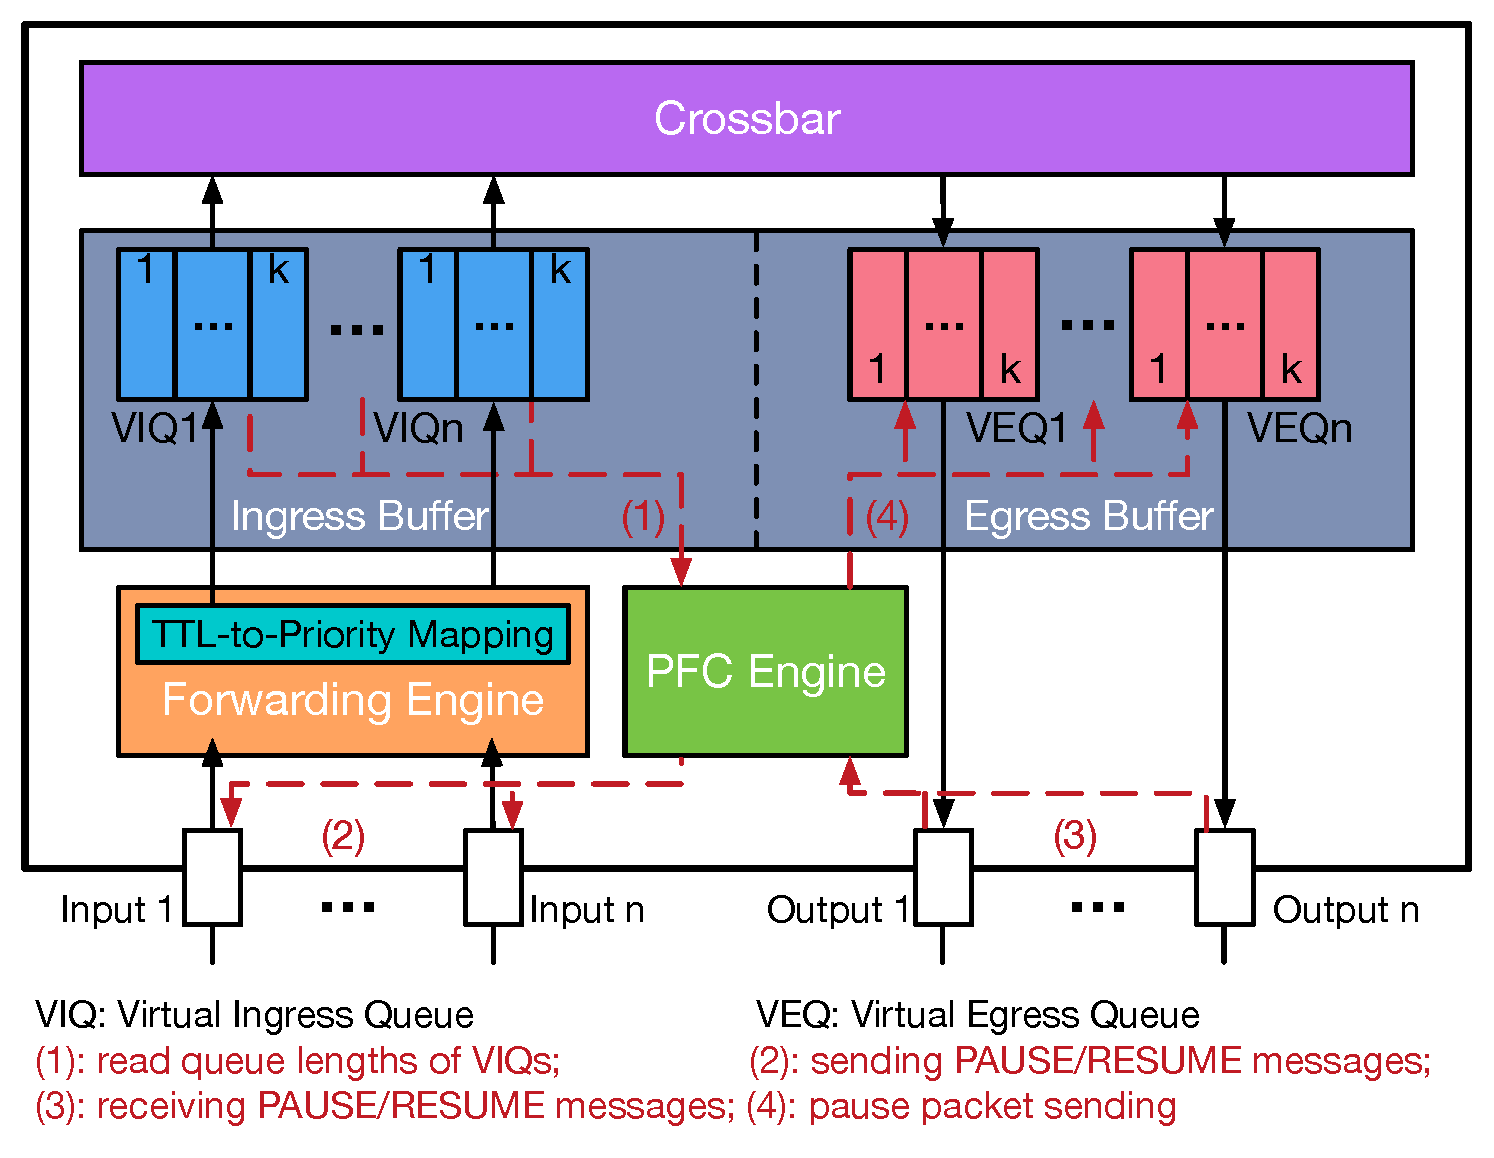
\includegraphics[width=0.5\textwidth] {figs/switch_model}
	\caption{Switch model.}\label{fig:switchmodel}

\end{figure}

In this part, we introduce the switch model under which we develop our TTL-based buffer management scheme. As shown in Fig.~\ref{fig:switchmodel},
our switch model consists of five elements: switch port, forwarding engine, PFC engine, crossbar and switch buffer. The function of these elements are list as follows.

%Fig.~\ref{fig:switchmodel}(a) shows the architecture of the switch model, which consists of a switching fabric and N line cards. Line cards are mainly used to receive/send packets and make routing/forwarding decisions. Switching fabric is a module to transfer packet cells from the input line card to the output line card. 

\begin{itemize}
	\item \textbf{Switch port}: The element to receive and send packets. Each switch port consists of an input port and an output port, and is connected with a link.
	
	\item \textbf{Forwarding engine}: The element to make the routing and/or switching decisions. In the forwarding engine, there is a module to decide the priority class of a packet based on the TTL value. 
	
	\item \textbf{PFC engine}: The element to perform PFC function.
	
	\item \textbf{Crossbar}: The element to switch packet cells from the ingress buffer to the egress buffer. 
	
	\item \textbf{Switch buffer}: The element to buffer incoming packets. We assume shared buffer in our model. In the ingress buffer, we use  virtual ingress queue (VIQ) to track the incoming packets. In the egress buffer, we use virtual egress queue (VEQ) to track the outgoing packets. Each VIQ is uniquely corresponding to an input port, while each VEQ is uniquely corresponding to an output port. As shown in Fig.~\ref{fig:switchmodel}, both VIQ and VEQ consist of k queues, with each queue corresponding to a priority class. A packet of priority class $j$ will enter the $j$-$th$ queue of its destined VIQ and VEQ.
	
%    Note that in our switch model, when a packet in some VIQ is forwarded to some VEQ, this VIQ will not perform dequeue operation. Dequeue operation will be performed only after this packet leaves the switch buffer. This is because the purpose of using VIQ is to track the bytes of currently buffered packets received by an input port, such that PFC can work properly.
	
	\textbf{Discussion}: It is not always the case for switch to have both ingress buffer and egress buffer at the same time. It depends on the buffering strategy. If we adopt output-queued strategy, there will be no ingress buffer, and VIQs are simply some counters to record the bytes of buffered packets received by different input ports. If we adopt input-queued strategy~\cite{islip}, there will be no egress buffer, and VEQs can be simulated using virtual output	queuing technique~\cite{tinytera} at the ingress buffer. If we adopt the combined-input-and-output-queued strategy~\cite{chuang1999matching}, the switch will have both ingress buffer and egress buffer. The switching function of crossbar can also be virtual, not necessary to involve packet copying.

\end{itemize}

\textbf{Enqueue and dequeue operations of VIQ and EIQ}: We use $q_{in}^{i}$ to denote VIQ $i$, and $q_{out}^{i}$ to denote VEQ $i$.
Let $q_{in}^{i,j}$ be the $j$-$th$ queue of VIQ $i$, and $q_{out}^{i,j}$ be the $j$-$th$ queue of VEQ $i$ ($1\leq i \leq n$, $1 \leq j \leq k$). The dequeue and enqueue operatons of VIQ and VEQ are performed as follows:
	
	\begin{enumerate}
		\item  Packet $p$ of priority class $j$ enters the switch buffer via input port $i_1$: VIQ $i_1$ performs enqueue operation and puts packet $p$ to the tail of $q_{in}^{i_1,j}$.
		
		\item  Packet $p$ in the head of $q_{in}^{i_1,j}$ is forwarded to VEQ $i_2$:  VEQ $i_2$ performs enqueue operation and puts packet $p$ to the tail of $q_{out}^{i_2,j}$. At the same time, head point of $q_{in}^{i_1,j}$ is moved to the next packet currently queued in $q_{in}^{i_1,j}$. Note that dequeue operation of packet $p$ will not be performed at $q_{in}^{i_1,j}$ at this point in time. 
		
		\item  Packet $p$ in the head of $q_{out}^{i_2,j}$ is forwarded to output port $i_2$: VEQ $i_2$ performs dequeue operation and removes packet $p$ from $q_{out}^{i_2,j}$.  VIQ $i_1$ performs dequeue operation and removes packet $p$ from $q_{in}^{i_1,j}$ (say packet $p$ was previously forwarded from $q_{in}^{i_1,j}$ to $q_{out}^{i_2,j}$). 
	\end{enumerate}
		
	Note that in our switch model, dequeue operation is performed at corresponding VIQ only after packet $p$ leaves the switch buffer. This is because the purpose of using VIQ is to track the bytes of currently buffered packets received by an input port, such that PFC can work properly.

\subsection{Modified PFC Mechanism}\label{subsec:PFC}

As shown in Fig.~\ref{fig:switchmodel}(b), the function of our modified PFC mechanism consists of four parts. 

The PFC engine will track the instant queue lengths of all the VIQs (function (1)). If the queue length of some queue  $q_{in}^{i,j}$ exceeds the configured PFC threshold, PFC engine will generate a PAUSE message to pause the packet transmission of the immediate upstream node on priority class $j$-$1$ over the link connected with port $i$. If the queue length of $q_{in}^{i,j}$ becomes less than the threshold later, PFC engine will generate a RESUME message to resume the packet transmission over the previously paused link on priority class $j$-$1$ (function (2)).

If some output port, say output port $i$, receives a PAUSE or RESUME message on priority class $j$ from its immediate downstream node, the PFC engine will then pause or resume the corresponding egress queue $q_{out}^{i,j}$, accordingly (function (3) and function (4)).

The main difference between our modified PFC mechanism and the typical PFC mechanism is that, if the queue length of some queue $q_{in}^{i,j}$ at some network node exceeds the PFC threshold, PFC engine will pause the packet transmission of the immediate upstream node on priority class $j$-$1$ over the incoming link instead of on priority class $j$. This feature is important for realizing our TTL-based buffer management scheme, as we will introduce in the next.


\subsection{TTL-based Buffer Management Scheme}\label{subsec:ttlscheme}

\textbf{Buffer division}: we divide the buffer of network nodes into $k$ partitions, and let the $j$-$th$ partition associated with priority class $j$. If a packet is classified into priority class $j$, it will  be buffered in the $j$-$th$ buffer partition. Packets queued in queues $q_{in}^{i,j}$ and $q_{out}^{i,j}$ ($1\leq i \leq n$) are the packets currently buffered in the $j$-$th$ buffer partition.

Let $d$ be the number of hops of the longest legal routing path in the network, $n$ be the number of switch ports, and $m_{p}$ be the maximum packet size. Our buffer division will always ensure $k \geq d$, and the size of any buffer partition is no smaller than $n*m_{p}$. 

\textbf{TTL-based packet buffering}: 
\begin{enumerate}
	\item  Initially, we set the TTL values of all packets to $ttl_0=d$ at all the source servers. TTL value of every packet will be decreased by 1 per hop. At all the source servers, packets are buffered in a buffer of priority class $0$.
	
	\item Let $ttl_i$ be the TTL value of a packet $p$ at its $i$-$th$ hop ($i \geq 0$). If $ttl_i = 0$, packet $p$ will be dropped by the receiving switch or server. At every hop, the priority class of any incoming packet $p$ is calculated as $\lambda_p = ttl_0 - ttl_i $. Packet $p$ will be buffered and queued according to the calculated priority class $\lambda_p$ at every hop.
\end{enumerate}

\subsection{Proof of Deadlock-free Property}\label{subsec:proof}
In this part, we are going to prove that our TTL-based solution is deadlock-free regardless of the packet scheduling algorithms.

In our proof, we use $p_{size}$, $p_{ttl}$ and $p_{dst}$ to denote the size, the TTL value and the destination of a packet $p$, respectively. Any ingress queue $q_{in}^{i,j}$ and any egress queue $q_{out}^{i,j}$ are viewed as packet sets. According to the switch model, we have $q_{in}^{i}=\cup_{j=1}^{k}q_{in}^{i,j}$, and $q_{out}^{i}=\cup_{j=1}^{k}q_{out}^{i,j}$.

We use $|q_{in}^{i,j}|$ and $|q_{out}^{i,j}|$ to denote the queue lengths of $q_{in}^{i,j}$ and $q_{out}^{i,j}$, where $|q_{in}^{i,j}|=\sum_{p\in q_{in}^{i,j}}p_{size}$, and $|q_{out}^{i,j}|=\sum_{p\in q_{out}^{i,j}}p_{size}$.
\subsubsection{Definition of switch functions}
 
\begin{enumerate}
	
	\item \textbf{Packet scheduling function of VIQs $f^{in}_{sche}$:} This is the switch function to decide which packet currently queued in some VIQ $q_{in}^{i}$ to be processed at first. Formally, this function can be expressed as follows. 
	\begin{align} \label{eqn:inschedule}
	 f^{in}_{sche}: q_{in}^{i} \longrightarrow p \in q_{in}^{i}
	\end{align}
	
	\item \textbf{Packet scheduling function of VEQs $f^{out}_{sche}$:} This is the switch function to decide which packet currently queued in some VEQ $q_{out}^{i}$ to be processed at first. Formally, this function can be expressed as follows. 
	\begin{align} \label{eqn:outschedule}
	f^{out}_{sche}: q_{out}^{i} \longrightarrow p \in q_{out}^{i}
	\end{align}
	
	\item \textbf{Packet forwarding function $ f_{fwd}$:} This is the switch function to forward a packet from a VIQ to a VEQ. Formally, this function can be expressed as follows. 
	\begin{align} \label{eqn:fwd}
	 &	f_{fwd}: (q_{in}^{i_1,j}, q_{out}^{i_2,j}, p\in q_{in}^{i_1,j})  \longrightarrow \nonumber \\
	 	&\begin{cases}
	 	 q_{in}^{i_1,j}=q_{in}^{i_1,j}-\{p\},  \text{current node is destination of } p,\\
	     q_{out}^{i_2,j}=q_{out}^{i_2,j}\cup\{p\}, \text{otherwise.} 
	 	\end{cases}
	\end{align}
	
	
	\item \textbf{Packet transmission function $ f_{trans}$:} This is the switch function to send a packet from the VEQ of current network device to the VIQ of the immediate downstream device. Formally, this function can be expressed as follows:
	\begin{align} \label{eqn:trans}
	f_{trans}: &(q_{in}^{i_1, j}, q_{out}^{i_2, j}, q_{in}^{i_3, j+1}, p\in q_{in}^{i_1,j}\cap q_{out}^{i_2,j})  \longrightarrow  \nonumber \\
 &	(q_{in}^{i_1,j}=q_{in}^{i_1,j}-\{p\}, q_{out}^{i_2,j}=q_{out}^{i_2,j}-\{p\}, \nonumber \\ 
 &	 q_{in}^{i_3,j+1}=q_{in}^{i_3,j+1}\cup\{p\}),  \nonumber \\
 & \text{if } p_{ttl} > 0   
 	\end{align}
 	\begin{align} 
 	f_{trans}: &(q_{in}^{i_1, j}, q_{out}^{i_2, j}, p\in q_{in}^{i_1,j}\cap q_{out}^{i_2,j})  \longrightarrow  \nonumber \\
 	&(q_{in}^{i_1,j}=q_{in}^{i_1,j}-\{p\}, q_{out}^{i_2,j}=q_{out}^{i_2,j}-\{p\}), \nonumber \\ 
 	& \text{if } p_{ttl} =0
	\end{align}
	Note that here  $q_{in}^{i_1, j}$ and $q_{out}^{i_2,j}$ are two queues belonging to the same network node, while $q_{in}^{i_3, j+1}$ is a queue belonging to an immediate downstream network node.
\end{enumerate}


\subsubsection{Assumptions}

Let $t_{cost}(f)$ be the time cost of performing switch function $f$. In the following part, we list several assumptions we make in our proof.

\begin{enumerate}
	\item \textbf{PFC threshold is no smaller than maximum transmission unit (MTU):} Formally, we have $t_{PFC}\ge s_{MTU}$.
	
	\item \textbf{Finite packet scheduling time:} We assume that packet scheduling functions can decide the next packet to be processed within finite time. Formally, $f^{in}_{sche}$ and $f^{out}_{sche}$ should satisfy the following constraints at any network node:
		\begin{align} 
    	t_{cost}(f^{in}_{sche}(q_{in}^{i})) < \infty ,1\leq i \leq n \label{eqn:schecon1}\\
	    t_{cost}(f^{out}_{sche}(q_{out}^{i})) < \infty, 1\leq i \leq n \label{eqn:schecon2}
		\end{align}
		
	\item \textbf{No selection of duplicated packet:} the packet scheduling function $f^{in}_{sche}$ will not select the same packet twice. Formally, 
		\begin{align} \label{eqn:nodupschedule}
		f^{in}_{sche}: \quad& q_{in}^{i_1} \longrightarrow p \in q_{in}^{i_1}, \nonumber \\
		\mbox{Subject to}: \quad&1\leq i_2 \leq n, \forall p\prime \in q_{out}^{i_2}, p \neq p\prime .
		\end{align}
		
	\item \textbf{Prefering non-paused packet:} We assume $f^{out}_{sche}$ will always prefer non-paused packets over paused packets.
		
	\item \textbf{Finite packet forwarding time:} We assume that any packet can be forwarded from a VIQ to a VEQ within finite time. Formally, $f_{fwd}$ should satisfy the following constraint:
	    \begin{align} \label{eqn:fwdcon}
		t_{cost}(f_{fwd}((q_{in}^{i_1,j}, q_{out}^{i_2,j}, p\in q_{in}^{i_1,j}))) < \infty, \nonumber \\
		1\leq i_1, i_2 \leq n
		\end{align}
		
	\item \textbf{Finite packet transmission time when no PFC pause:} We assume that any packet can be sent to the VIQ of next hop within finite time when the priority class of the packet is not paused by the immediate downstream device. Formally, $f_{trans}$ should satisfy the following constraint:
	
	\begin{align} \label{eqn:transcon}
	t_{cost}(f_{trans}(q_{in}^{i_1, j}, q_{out}^{i_2, j}, q_{in}^{i_3, j+1}, p\in q_{in}^{i_1,j}\cap q_{out}^{i_2,j}))= \nonumber \\
	\begin{cases}
	<\infty, &\quad |q_{in}^{i_3,j+1}|< t_{PFC}\\
	\infty, &\quad\text{otherwise.} \ 
	\end{cases}
	\end{align}
	
    \end{enumerate}
    
    
   \subsubsection{Network Buffer State}
   
   \textbf{Buffer state:} we use a $2n$ dimensional vector  to represent the buffer state of a network node $u$ as follows: 
   \begin{align}
   BS_u=<q_{in}^{1}, \dots, q_{in}^{n}, q_{out}^{1}, \dots,q_{out}^{n}> \nonumber 
   	\end{align}
   	$BS_u(t)$ is the buffer state of node $u$ at time $t$.
   
   Let $N(V,E)$ be the network topology, where $V$ is the set of network nodes and $E$ is the set of network links. We represent the buffer state of netwrok $N$ (denoted as $BS_N$) as follows:
   \begin{align}
   BS_N=<BS_{u_1},\dots,BS_{u_i},\dots>,\forall u_i \in V \nonumber 
   \end{align}
   $BS_N(t)$ is the buffer state of network $N$ at time $t$.
   
   \textbf{Legal buffer state:} We say $BS_u$ is a legal buffer state for node $u$ when the following two conditions are satisfied:
   \begin{align} \label{eqn:legalstatecon}
    |q_{in}^{i}|<\infty\quad  \text{and}\quad   |q_{out}^{i}|<\infty, \quad 1\leq i \leq n
%    |q_{in}^{i,j}|\leq t_{PFC}, \quad 1\leq i \leq n, 1\leq j \leq k \label{eqn:legalstatecon2}
   \end{align}
   
   We say $BS_N$ is a legal buffer state when the buffer state of every node in $N$ is legal.
   
   \textbf{Empty buffer state:} We say $BS_u$ is an empty buffer state when the following condition is satisfied:
    \begin{align} \label{eqn:emptystatecon}
    |q_{in}^{i}|=0\quad  \text{and}\quad   |q_{out}^{i}|=0, \quad 1\leq i \leq n 
    \end{align}
    
    We say $BS_N$ is a empty buffer state when the buffer state of every node in $N$ is empty. Specially, we denote the empty buffer state of network $N$ as $BS^0_N$.
    
  \textbf{Deadlocked buffer state:} $\forall t< \infty$, we say $BS_N(t)$ is a deadlocked buffer state if the following condition is met when no new packets are injected into the network since $t$:
  \begin{align} \label{eqn:deadlockstatedef}
  \exists \text{ finite } t_0 > t, \quad \forall t_1>t_0, \nonumber\\
  BS_N(t_1)\equiv BS_N(t_0) \quad \text{and} \quad BS_N(t_0) \neq BS^0_N.
  \end{align}
  
    \subsubsection{Proof of deadlock-free}
    

    
    \textbf{Claim:} our TTL-based solution is deadlock-free regardless of the packet scheduling algorithms.
  
    \textbf{Proof:} To prove our TTL-based solution is deadlock-free, we prove by contradiction that no legal buffer state can be deadlocked buffer state under our TTL-based solution.
    
    Assuming there exists a legal buffer state  $BS_N(t)$ which is also a deadlocked buffer state under our TTL-based solution. If no new packets are injected into the network since $t$, according to Equation~(\ref{eqn:deadlockstatedef}), $BS_N(t)$ will converge into a fixed non-empty buffer state $BS_N(t_0)$ at some finite time $t_0>t$. 
    
    
   \textbf{Case 1:} All the VEQs in $BS_N(t_0)$ is empty. As $BS_N(t_0) \neq BS^0_N$, $BS_N(t_0)$ has at least one non-empty VIQ. As $BS_N(t)$ is a legal buffer state, accroding to Equation~(\ref{eqn:legalstatecon}), there are finite number of packets queued in non-empty VIQs of $BS_N(t_0)$. Then according to Equations~(\ref{eqn:schecon1}), (\ref{eqn:nodupschedule}) and (\ref{eqn:fwdcon}), any unscheduled packet remaining in any VIQ will be forwarded to some VEQ within finite time at some finite time $t_2>t_0$. This means that $BS_N(t_0)$ will transition to some other buffer state, which violates the fact that $\forall t_1>t_0, BS_N(t_1)\equiv BS_N(t_0)$.
   
   \textbf{Case 2:} There exist some non-empty VEQs (at least one) in $BS_N(t_0)$. Let $q_{out}^{i,m}$ be the queue of highest priority class among all the non-empty VEQ queues ($m\leq k$). Under our TTL-based solution, packets in $q_{out}^{i,m}$ will not be paused by PFC PAUSE messages as packets can only be paused by packets of higher priority class. According to Equations~(\ref{eqn:schecon2}) and (\ref{eqn:transcon}), packets in $q_{out}^{i,m}$ will be transmitted to next hop within finite time. This means that $BS_N(t_0)$ will transition to some other buffer state  at some finite time $t_2>t_0$, which violates the fact that $\forall t_1>t_0, BS_N(t_1)\equiv BS_N(t_0)$.
   
   Based on the above discussion, the assumption we made will cause contradiction in both cases. Hence $BS_N(t)$ is not a deadlocked buffer state under our TTL-based solution. So our TTL-based solution is deadlock-free regardless of the packet scheduling algorithms.
    
    
    
    %     \textbf{Lemma 1}: for arbitrary non-deadlocked buffer state $BS_N(t)$, when no new packets are injected into the network since $t$, there exists a finite $t_0>t$, $BS_N(t_0)=BS^0_N$.
    %     
    %      \textbf{Proof}: Assuming that there does not exist a finite $t_0>t$, $BS_N(t_0)=BS^0_N$. As $BS_N(t)$ is a non-deadlocked buffer state, according to Equation~\ref{eqn:deadlockstatedef}, $BS_N(t)$ will not converge into any fixed non-empty buffer state. 
    %      
    %      Let $BS_N(t_1), \dots, BS_N(t_i), \dots$ be the buffer states $BS_N(t)$ will transition to in sequence since $t$. Let $Sum_{TTL}(BS_N(t))$ be the sum of TTL values of all packets 
    %      
    %      We consider any transition from $BS_N(t_i)$ to $BS_N(t_{i+1})$, $i>0$,
    %      
    %      \textbf{}
    
%\textcolor{red}{To be added.}

%In this part, we will prove that our solution can ensure a \textit{lossless} network and at the same time is \textit{deadlock-free} when the following four assumptions are met.
%
%\textbf{Assumption 1}: There is no transmission or processing errors at all the network nodes.
%
%\textbf{Assumption 2}: PFC PAUSE/RESUME messages can take effect immediately at the corresponding upstream node, i.e., there is no link delay and processing delay.
%
%\textbf{Assumption 3}: The scheduling algorithm of any VIQ is deadlock-free: for any given time $t$, any packet $p$ queued in arbitrary $q_{in}^{i,j}$, $1\leq i \leq n$, $1 \leq j \leq k$, can be forwarded to the destined VEQ within some finite time since $t$.
%
%\textbf{Assumption 4}: The scheduling algorithm of any VEQ is deadlock-free: for any given time $t$, any packet $p$ queued in arbitrary $q_{out}^{i,j}$, $1\leq i \leq n$, $1 \leq j \leq k$, can be forwarded to next hop's VIQ via output port $i$ within some finite time since $t$, as long as two conditions are met: 1) $q_{out}^{i,j}$ is not paused by PFC PAUSE message since $t$; 2) VEQ $i$ does not receive any new packets since $t$.
%
%\textbf{Claim 1}: The TTL based buffer management scheme can work with the modified PFC mechanism to ensure a lossless network.
%
%\textbf{Claim 2}: The network is deadlock-free after applying the TTL based buffer management scheme and the modified PFC mechanism.
%
%To prove the above two claims, we first present two lemmas.
%
%\textbf{Lemma 1}: The priority class $\lambda_p$ of a packet $p$ buffered at a given node always satisfies $\lambda_p \leq d$.
%
%\textit{Proof}: As a packet with TTL value equal to 0 will be dropped by the received node, we have $ttl_i \geq 0$. Then we have $\lambda_p = ttl_0 - ttl_i \leq ttl_0 - 0 = d$.
%
%\textbf{Lemma 2}: If we stop injecting new packets into the network since some time $t_0$, arbitrary $q_{out}^{i,j}$, $1\leq i \leq n$, $1 \leq j \leq k$, will become empty within some finite time since $t_0$. 
%
%\textit{Proof}: We use induction on $\lambda_p$ to prove the lemma. First, we consider $\lambda_p=d$. 
%
%Under our modified PFC mechanism, pacekts in $q_{in}^{i,j}$ of some node are only possible to pause the packet transmission of the immediate upstream node on priority class $j$-$1$.  So packets in any $q_{out}^{i,j}$ of one node are only possible to be paused by the packets of higher priority class at some immediate downstream node. According to Lemma 1,  $q_{out}^{i,d}$ is the queue of highest priority class among all the non-empty queues. Hence packets in $q_{out}^{i,d}$ will not be paused by PFC PAUSE messages. 
%
%In the next, we prove by contradiction that any packet in $q_{out}^{i,d}$ can get drained within some finite time since $t_0$. We first assume that there exists a packet $p$ in $q_{out}^{i,d}$ which cannot get drained within some finite time since $t_0$. According to Assumption 4, if the following two conditions are met, packet $p$ will get drained within some finite time: (1) $q_{out}^{i,d}$ is not paused by PFC PAUSE messages; and (2) there exists a finite time $t_1>t_0$,  since which no new packets will be forwarded to VEQ $i$. The first condition is already met. To make our assumption valid, we can conclude that there does not exist a finite time $t_1>t_0$,  since which no new packets will be forwarded to VEQ $i$.
%
%As no new packets are injecting into the network since $t_0$, the number of packets remaining in the network is finite (denoted as $N_p$). Further, any packet traversing more than $d$ hops in the network will be dropped. Therefore, the number of packets to be forwarded to VEQ $i$ since $t_0$ is finite (no larger than $N_p*d$). 
%
%Let $t_1$ be the time at which the last packet is forwarded to VEQ $i$. $t_1$ must be finite as there are only finite number of packets to be forwarded to VEQ $i$. This contradicts with the conclusion that there does not exist a finite time $t_1>t_0$,  after which no new packets are forwarded to VEQ $i$. So our previous assumption is not valid. Then we can conclude that any packet in $q_{out}^{i,d}$ can get drained within some finite time since $t_0$.
%
%Since (1) any packet in $q_{out}^{i,d}$ can get drained within some finite time since $t_0$ and (2) the number of packets to be forwarded to VEQ $i$ since $t_0$ is finite, $q_{out}^{i,j}$ will become empty within some finite time since $t_0$. 
%
%Next, we show that the lemma holds for $\lambda_p=d-1$. After $q_{out}^{i,j}$ becomes empty at all the nodes, $q_{out}^{i,d-1}$ becomes the queue of highest priority class among all the non-empty queues. Following the same analysis, we can know that $q_{out}^{i,d-1}$ will become empty within some finite time since $t_0$. This completes proof of the lemma.
%
%
%\textbf{Proof of Claim 1}: Let $b_j$ be the buffer size of the $j$-$th$ buffer partition. At every switch and every server, we set the PFC threshold of priority class $j$ as $b_j-n*m_{max}$.
%
%At any given time $t$, we consider packet $p$ in the head of arbitrary $q_{out}^{i,j}$, $1\leq i \leq n$, $1 \leq j \leq k$. 
%
%Case 1: $q_{out}^{i,j}$ is not paused by PFC PAUSE messages at time $t$. According to the PFC threshold, at the immediate downstream node, the remaining buffer size of the ($j$+$1$)-$th$ buffer partition will be no smaller than $n*m_{p}$, where $n$ is the number of switch ports and $m_{p}$ is the maximum packet size.  In the worst case, when packet $p$ is being sent to the immediate downstream node, other $n$-$1$ packets are being sent to the same node over different input ports at the same time. As the remaining buffer is large enough to accommodate all these $n$ packets, packet $p$ will not be dropped.
%
%case 2: $q_{out}^{i,j}$ is paused by PFC PAUSE messages at time $t$. In this case, packet $p$ will not be dropped as it is paused.
%
%In the above analysis, the consideration of packet $p$ and time $t$ is arbitrary, so no packet will be dropped at any node under our solution. So our solution can ensure a lossless network when properly setting the PFC threshold.
%
%\textbf{Proof of Claim 2}: For arbitrary given time $t$, in order to know whether the network is already in a state of deadlock, we can stop the injection of new packets into the network at time $t$, and observe whether all the packets remaining in the network can get drained within some finite time. 
%
%According to Lemma 2, under our TTL-based buffer management scheme, if we stop the injection of new packets into the network at time $t$, all VEQs will become empty within some finite time since $t$. According to Assumption 3, no packet will be permanently buffered in the VIQs. So packets in VIQs can also get drained within some finite time. Therefore, all the packets remaining in the network can get drained within some finite time. 
%
%Based on the above discussion, our TTL-based buffer management scheme is deadlock-free.

